\begin{frame}{DPA vs. SPA}
    \begin{itemize}
        \item We have seen that SPA analyzes leakages along the time axis, exploiting relationships between leakages and operations.
       \item DPA, on the other hand, exploits the relationship between leakages at specific time samples and the data being processed in the DUT.
       \item Compared to SPA, DPA does not require detailed knowledge about the implementation.
        \item Normally it suffices to know what cryptographic algorithm is being executed in the DUT.
    \end{itemize}
\end{frame}

\begin{frame}{Attack assumption}
    \begin{itemize}
        \item In our DPA attacks, we assume the attacker has the knowledge of the plaintext and the goal is to recover the very first round key of a symmetric block cipher -- for some ciphers, e.g. PRESENT-80, this is the first round key; for some ciphers, e.g. AES-128, this is the whitening key, which is equal to the master key.
        \item Similar attack strategies apply if we assume the attacker has the knowledge of the ciphertext and aims to recover the last round key.
    \end{itemize}
\end{frame}


\begin{frame}{PRESENT -- encryption}
\begin{columns}[T] % align columns
\begin{column}{.55\textwidth}
\begin{itemize}
     \item block length: $n=64$
       \item number of rounds: \texttt{Nr}$=31$
       \item key length: either $80$ or $128$.
    \item Round function: addRoundKey, sBoxLayer, and pLayer.
    \item After $31$ rounds, addRoundKey is applied again before the ciphertext output 
\end{itemize}
\begin{alertblock}{Remark}
    For PRESENT specification, we consider the $0$th bit of a value as the rightmost bit in its binary representation.
For example, the $0$th bit of $3=011_2$ is $1$, the $1$st bit is $1$ and the $2$nd bit is $0$.
\end{alertblock}
\end{column}%
\hfill%
\begin{column}{.5\textwidth}
\begin{figure}
    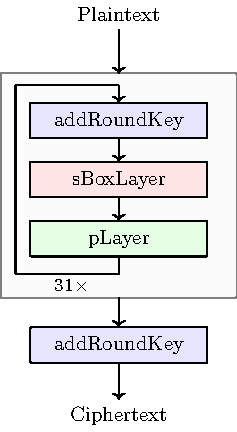
\includegraphics[width=0.6\textwidth]{fig/PRESENT.pdf}
\end{figure}
\end{column}%
\end{columns}
\end{frame}

\begin{frame}{PRESENT -- addRoundKey}
    \begin{itemize}
        \item Round key $K_i=\kappa^i_{63}\dots\kappa_0^i$, $(1\leq i\leq 32)$
        \item Current state $b_{63}b_{62}\dots b_0$
        \item For $0\leq j\leq 63$
    \end{itemize}
    \[
b_j\to b_j\oplus\kappa_j^i
\]
\end{frame}

\begin{frame}{PRESENT -- sBoxLayer}
    \begin{itemize}
        \item sBoxLayer applies sixteen $4-$bit Sboxes to each nibble of the current cipher state.
        \item For example, if the input is \texttt{0}, the output is \texttt{C}.
\begin{table}[htb]
\centering
\ttfamily
\begin{tabular}{cccccccccccccccc}\hline
 0 & 1 & 2 & 3 & 4 & 5 & 6 & 7 & 8 & 9 & A & B & C & D & E & F \\\hline
 C & 5 & 6 & B & 9 & 0 & A & D & 3 & E & F & 8 & 4 & 7 & 1 & 2\\\hline
\end{tabular}
\end{table}
    \end{itemize}
\end{frame}


\begin{frame}{PRESENT -- pLayer}
pLayer permutes the $64$ bits using the following formula:
\[
\text{pLayer}(j)=\left\lfloor\frac{j}{4}\right\rfloor+(j\mo 4)\times16,
\]
where $j$ denotes the bit position.
\begin{table}[htb]
\centering
\begin{tabular}{cccccccccccccccc}\hline
0 & 1 & 2 & 3 & 4 & 5 & 6 & 7 & 8 & 9 & 10 & 11 & 12 & 13 & 14 & 15 \\
0 & 16 & 32 & 48 & 1 & 17 & 33 & 49 & 2 & 18 & 34 & 50 & 3 & 19 & 35 & 51 \\\hline
16 & 17 & 18 & 19 & 20 & 21 & 22 & 23 & 24 & 25 & 26 & 27 & 28 & 29 & 30 & 31 \\
4 & 20 & 36 & 52 & 5 & 21 & 37 & 53 & 6 & 22 & 38 & 54 & 7 & 23 & 39 & 55 \\\hline
32 & 33 & 34 & 35 & 36 & 37 & 38 & 39 & 40 & 41 & 42 & 43 & 44 & 45 & 46 & 47 \\
8 & 24 & 40 & 56 & 9 & 25 & 41 & 57 & 10 & 26 & 42 & 58 & 11 & 27 & 43 & 59 \\\hline
48 & 49 & 50 & 51 & 52 & 53 & 54 & 55 & 56 & 57 & 58 & 59 & 60 & 61 & 62 & 63 \\
12 & 28 & 44 & 60 & 13 & 29 & 45 & 61 & 14 & 30 & 46 & 62 & 15 & 31 & 47 & 63\\\hline
\end{tabular}
\end{table}
\end{frame}

\begin{frame}{Two rounds of PRESENT}
    \begin{itemize}
        \item For our DPA attacks, we will attack the $0$th Sbox and try to recover one nibble of the first round key
    \end{itemize}
    \begin{figure}
    \centering
    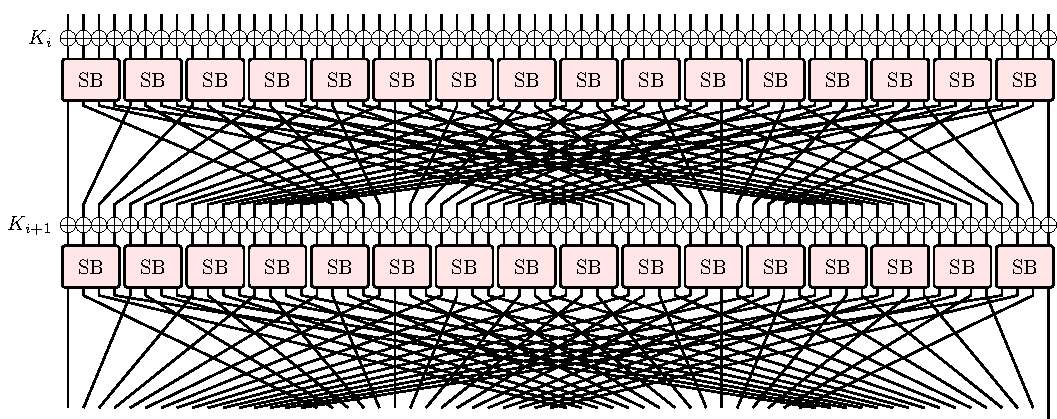
\includegraphics[width=0.9\textwidth]{fig/PRESENT_two_rounds.pdf}
\end{figure}
\end{frame}

\begin{frame}{DPA attack -- step 1}
\textbf{Identify the target cryptographic implementation}
    \begin{itemize}
        \item DPA attacks can be applied to unprotected implementations of any symmetric block cipher that has been proposed so far.
    \end{itemize}
    \begin{example}
        As a running example, we will look at the computation of PRESENT.
    \end{example}
\end{frame}

\begin{frame}{DPA attack -- step 2}
\textbf{Experimental setup and measure leakages}
    \begin{itemize}
        \item The efficiency and success of the attack are highly dependent on the measurement devices the attacker has access to.
        \item Suppose we have taken measurements of the target implementation with $M_p$ plaintexts.
       \item For $j=1,\dots,M_p$, let $\boldsymbol{\ell}_j=(l^{j}_1,
    l^{j}_2,\dots,l^j_q)$ denote the corresponding power trace, where $q$ is the total number of time samples in one trace.
    \end{itemize}
    \begin{example}
    We will use the \dataranone as illustrations.
        \begin{itemize}
                \item Each trace has $3600$ time samples
                \item Contains 5000 traces with a fixed round key \texttt{0xFEDCBA0123456789} and a random plaintext for each trace.
            \item In particular, we have $M_p=5000$, $q=3600$.
        \end{itemize}
    \end{example}
\end{frame}

\begin{frame}{DPA attack -- step 3}
    \textbf{Choose the part of the key to recover}
    \begin{itemize}
        \item DPA attack is normally carried out in a divide-and-conquer manner.
       \item We focus on a small part (e.g. a nibble, a byte) of a round key in each attack and each part of the round key can be recovered independently.
       \item With the inverse key schedule, one (e.g. AES) or two round keys (e.g. PRESENT, DES) will reveal the master key
      \item Let $k$ denote the target part of the key and let $M_k$ denote the number of possible values of $k$.
    \end{itemize}
    \begin{example}
        For our attack example, we will focus on the $0$th nibble of the first round key for PRESENT and $M_k=16$.
    \end{example}
\end{frame}

\begin{frame}{DPA attack -- step 4}
\textbf{Choose the target intermediate value}
    \begin{itemize}
        \item To recover the key, we exploit relationships between leakages and a certain intermediate value being processed in the DUT.
       \item The goal is to gain information about this intermediate value, which reveals information about our chosen part of the key.
      \item  Let $\boldsymbol{v}$ denote the target intermediate value.
   \item We require that there is a function $\varphi$, such that
    \[
    \boldsymbol{v}=\varphi(k,p),
    \]
    where $p$ denotes (part of) the plaintext.
    \end{itemize}
    \begin{example}
    \begin{itemize}
        \item $k$: $0$th nibble of the first round key
        \item $\boldsymbol{v}$: $0$th Sbox output of the first round
        \item $p$: $0$th nibble of the plaintext
    \end{itemize}
    \[
    \boldsymbol{v}=\text{SB}_{\text{PRESENT}}(k\oplus p),
    \]
    \end{example}
\end{frame}

\begin{frame}{DPA attack -- step 5}
\textbf{Compute hypothetical target intermediate values}
    \begin{itemize}
        \item A small part of the key is related to our target intermediate value.
        \item We can make a guess of this part of the key and obtain a hypothetical value for our target intermediate value.
        \item In particular, for each key hypothesis $\hat{k}_i$ of $k$, and each (part of the) plaintext $p_j$, we can compute a hypothesis for $\boldsymbol{v}$, which is given by
    \[
    \hat{\boldsymbol{v}}_{ij}=\varphi(\hat{k}_i,p_j),\quad i=1,2,\dots,M_k,\quad j=1,2,\dots,M_p.
    \]
    \end{itemize}
    \begin{example}
    \begin{itemize}
    \item For our attacks, with each key hypothesis of the $0$th nibble of the first round key, we have a hypothetical value for the $0$th Sbox output:
    \[
    \hat{\boldsymbol{v}}_{ij}=\text{SB}_{\text{PRESENT}}(\hat{k}_i\oplus p_j),\quad i=1,2,\dots,16,\quad j=1,2,\dots,5000.
    \]
        \item  $p_j$ is the $0$th nibble of the plaintext corresponding to the attack trace $\boldsymbol{\ell}_j$.
        \item We set $\hat{k}_i=i-1,\quad i=1,2,\dots,16.$
    \end{itemize}
    \end{example}
\end{frame}

\begin{frame}{DPA attack -- step 5}
    \textbf{Compute hypothetical target intermediate values}
    \begin{table}[htb]
\centering
\ttfamily
\begin{tabular}{cccccccccccccccc}\hline
 0 & 1 & 2 & 3 & 4 & 5 & 6 & 7 & 8 & 9 & A & B & C & D & E & F \\\hline
 C & 5 & 6 & B & 9 & 0 & A & D & 3 & E & F & 8 & 4 & 7 & 1 & 2\\\hline
\end{tabular}
\end{table}
    \begin{example}
        For our attacks, with each key hypothesis of the $0$th nibble of the first round key, we have a hypothetical value for the $0$th Sbox output:
    \[
    \hat{\boldsymbol{v}}_{ij}=\text{SB}_{\text{PRESENT}}(\hat{k}_i\oplus p_j),\quad i=1,2,\dots,16,\quad j=1,2,\dots,5000.
    \]
    We set $\hat{k}_i=i-1,\quad i=1,2,\dots,16.$
    \begin{itemize}
    \item $\hat{k}_1=\texttt{0}$, $\hat{k}_2=\texttt{1}$.
    \item For \dataranone, we have $p_1=\texttt{9},\quad p_2=\texttt{C}.$
    \end{itemize}
    \end{example}
\end{frame}

\begin{frame}{DPA attack -- step 5}
    \textbf{Compute hypothetical target intermediate values}
    \begin{table}[htb]
\centering
\ttfamily
\begin{tabular}{cccccccccccccccc}\hline
 0 & 1 & 2 & 3 & 4 & 5 & 6 & 7 & 8 & 9 & A & B & C & D & E & F \\\hline
 C & 5 & 6 & B & 9 & 0 & A & D & 3 & E & F & 8 & 4 & 7 & 1 & 2\\\hline
\end{tabular}
\end{table}
    \begin{example}
    \[
    \hat{\boldsymbol{v}}_{ij}=\text{SB}_{\text{PRESENT}}(\hat{k}_i\oplus p_j),\quad i=1,2,\dots,16,\quad j=1,2,\dots,5000.
    \]
    \begin{itemize}
    \item $\hat{k}_1=\texttt{0}$, $\hat{k}_2=\texttt{1}$.
    \item $p_1=\texttt{9},\quad p_2=\texttt{C}.$
    \end{itemize}
      \begin{eqnarray*}
        \hat{\boldsymbol{v}}_{11}&=&\text{SB}_{\text{PRESENT}}(\hat{k}_1\oplus p_1)=\text{SB}_{\text{PRESENT}}(\texttt{0}\oplus\texttt{9})=\text{SB}_{\text{PRESENT}}(\texttt{9})=\texttt{E},\\
        \hat{\boldsymbol{v}}_{12}&=&\text{SB}_{\text{PRESENT}}(\hat{k}_1\oplus p_2)=\text{SB}_{\text{PRESENT}}(\texttt{0}\oplus\texttt{C})=\text{SB}_{\text{PRESENT}}(\texttt{C})=\texttt{4},\\
        \hat{\boldsymbol{v}}_{21}&=&\text{SB}_{\text{PRESENT}}(\hat{k}_2\oplus p_1)=\text{SB}_{\text{PRESENT}}(\texttt{1}\oplus\texttt{9})=\text{SB}_{\text{PRESENT}}(\texttt{8})=\texttt{3},\\
         \hat{\boldsymbol{v}}_{22}&=&\text{SB}_{\text{PRESENT}}(\hat{k}_2\oplus p_2)=\text{SB}_{\text{PRESENT}}(\texttt{1}\oplus\texttt{C})=\text{SB}_{\text{PRESENT}}(\texttt{D})=\texttt{7}.
    \end{eqnarray*}
    \end{example}
\end{frame}

\begin{frame}{DPA attack -- step 6}
    \textbf{Choose the leakage model}
    \begin{itemize}
        \item For each hypothetical target intermediate value, we can compute the hypothetical signal depending on our leakage model
    \[
    \mathcal{H}_{ij}:=\mathcal{L}(\hat{\boldsymbol{v}}_{ij})-\text{noise},\quad i=1,2,\dots,M_k,\quad j=1,2,\dots,M_p,
    \]
    \item We subtract the noise component from the leakage model.
    \end{itemize}
\end{frame}

\begin{frame}{Recall -- Leakage model}
    \begin{itemize}
        \item Assume a value $\boldsymbol{v}$ is being processed in the DUT
        \item Let $N\sim\mathcal{N}(0,\sigma^2)$ be a normal random variable with mean $0$ and variance $\sigma^2$.
        \item \textit{identity leakage model}
        \begin{itemize}
            \item the leakage is correlated to $\boldsymbol{v}$
            \[
\mathcal{L}(\boldsymbol{v})=\boldsymbol{v}+\text{noise},
\]
        \end{itemize}
        \item \textit{Hamming weight model}
        \begin{itemize}
            \item the leakage will then be correlated to $\wt{\boldsymbol{v}}$, the Hamming weight of $\boldsymbol{v}$\footnote{the Hamming weight of vector $\boldsymbol{v}\in\FF_2^m$ is defined to be the number of $1$s in $\boldsymbol{v}$}
            \[
    \mathcal{L}(\boldsymbol{v})=\wt{\boldsymbol{v}}+\text{noise}.
\]
        \end{itemize}
    \end{itemize}
    \begin{example}
    $\boldsymbol{v}=\texttt{A}$
    \begin{itemize}
        \item identity leakage model: $\mathcal{L}(\boldsymbol{v})=10+\text{noise}$
        \item Hamming weight leakage model: $\mathcal{L}(\boldsymbol{v})=2+\text{noise}$
    \end{itemize}
    \end{example}
\end{frame}

\begin{frame}{DPA attack -- step 6}
    \textbf{Choose the leakage model}
    \begin{itemize}
        \item For each hypothetical target intermediate value, we can compute the hypothetical signal depending on our leakage model
    \[
    \mathcal{H}_{ij}:=\mathcal{L}(\hat{\boldsymbol{v}}_{ij})-\text{noise},\quad i=1,2,\dots,M_k,\quad j=1,2,\dots,M_p,
    \]
    \item We subtract the noise component from the leakage model.
    \item Hamming weight leakage model
    \[
    \mathcal{L}(\boldsymbol{v})=\wt{\boldsymbol{v}}+\text{noise}.
    \]
    \item If we choose the Hamming weight leakage model, we have
    \[
    \mathcal{H}_{ij}=\wt{\hat{\boldsymbol{v}}_{ij}},\quad i=1,2,\dots,M_k,\quad j=1,2,\dots,M_p.
    \]
    \end{itemize}
\end{frame}

\begin{frame}{DPA attack -- step 6}
    \textbf{Choose the leakage model}
    \begin{itemize}
        \item For each hypothetical target intermediate value, we can compute the hypothetical signal depending on our leakage model
    \[
    \mathcal{H}_{ij}:=\mathcal{L}(\hat{\boldsymbol{v}}_{ij})-\text{noise},\quad i=1,2,\dots,M_k,\quad j=1,2,\dots,M_p,
    \]
    \item We subtract the noise component from the leakage model.
    \end{itemize}
    \begin{example}
    \[
    \hat{\boldsymbol{v}}_{11}=\texttt{E},\quad\hat{\boldsymbol{v}}_{12}=\texttt{4},\quad\hat{\boldsymbol{v}}_{21}=\texttt{3},\quad\hat{\boldsymbol{v}}_{22}=\texttt{7}.
    \]
    According to the Hamming weight leakage model:
    \[
    \mathcal{H}_{11}=\wt{\texttt{E}}=3,\quad\mathcal{H}_{12}=\wt{\texttt{4}}=1,\quad\mathcal{H}_{21}=\wt{\texttt{3}}=2,\quad\mathcal{H}_{22}=\wt{\texttt{7}}=3
    \]
    According to the identity leakage model:
    \[
    \mathcal{H}_{11}=\texttt{E}=14,\quad\mathcal{H}_{12}=\texttt{4}=4,\quad\mathcal{H}_{21}=\texttt{3}=3,\quad\mathcal{H}_{22}=\texttt{7}=7
    \]
    \end{example}
\end{frame}

\begin{frame}{What we have done so far}
    \begin{example}
    \begin{itemize}
        \item For our attacks, we aim to recover the $0$th nibble of the first round key for PRESENT encryption, denoted $k$
        \item The target intermediate value is the $0$th Sbox output
        \item $5000$ measurements, corresponding $0$th nibble of plaintext is $p_j$
        \item With each key hypothesis of $k$, we have a hypothetical value for $\boldsymbol{v}$:
        \[
    \hat{\boldsymbol{v}}_{ij}=\text{SB}_{\text{PRESENT}}(\hat{k}_i\oplus p_j),\quad i=1,2,\dots,16,\quad j=1,2,\dots,5000.
    \]
    \item With a chosen leakage model, we have a hypothetical signal
    \begin{itemize}
        \item Hamming weight leakage model: $\mathcal{H}_{ij}=\wt{\hat{\boldsymbol{v}}_{ij}}$
        \item Identity leakage mode: $\mathcal{H}_{ij}=\hat{\boldsymbol{v}}_{ij}$
    \end{itemize}
    \end{itemize}
    \end{example}
\end{frame}

\begin{frame}{DPA attack -- step 7}
\textbf{Statistical analysis}
\begin{itemize}
    \item For a fixed key hypothesis $\hat{k}_i$, we view the modeled signal as a random variable $\mathcal{H}_i$ that varies when the plaintext changes.
    \item If we fix a time sample $t$, we also consider the leakage at this time as a random variable $L_t$.
    \item We would like to know how good the modeled signals are compared to the actual leakages for each key hypothesis.
    \item For the correct key hypothesis and the time samples corresponding to POIs, we expect the modeled signals to be correlated to the real leakages.
\end{itemize}
\end{frame}

\begin{frame}{DPA attack -- step 7}
\textbf{Statistical analysis}
\begin{itemize}
    \item We adopt the notion of correlation coefficient.
    \item For each key hypothesis $\hat{k}_i$ ($i=1,2,\dots,M_k$) and each time sample $t$ ($t=1,2,\dots,q$), we compute the sample correlation coefficient, denoted by $r_{i,t}$, of $\mathcal{H}_i$ and $L_t$:
     \[
    r_{i,t}:=\frac{\sum_{j=1}^{M_p}(\mathcal{H}_{ij}-\overline{\mathcal{H}_i})(l_t^j-\overline{l_t})}{\sqrt{\sum_{j=1}^{M_p}(\mathcal{H}_{ij}-\overline{\mathcal{H}_i})^2}\sqrt{\sum_{j=1}^{M_p}(l_t^j-\overline{l_t})^2}},
    \]
    where $\overline{\mathcal{H}_i}$ and $\overline{l_t}$ are the means of $\mathcal{H}_i$ and $l_t$ respectively. And
    \[
    \overline{\mathcal{H}_i} = \frac{1}{M_p}\sum_{j=1}^{M_p}\mathcal{H}_{ij}.
    \]
    is the average of all hypothetical leakages for the same key hypothesis $\hat{k}_i$
    \item $\overline{l_t}$ can be obtained by taking all the leakages at time sample $t$ from all traces and compute the average
\end{itemize}
\end{frame}

\begin{frame}{DPA attack -- step 7}
    \begin{itemize}
        \item The target intermediate value $\boldsymbol{v}$ will be processed in our DUT at certain points in time -- the leakages at those corresponding time samples (POIs) should be correlated to $\boldsymbol{v}$.
        \item If a good leakage model (i.e. a model that is close to the actual leakage of the DUT) is chosen, we expect $\mathcal{H}_i$ and $L_t$ to be correlated for the correct key hypothesis $\hat{k}_i$ and POIs $t$.
      \item The key hypothesis that achieves the highest \textit{absolute value} of $r_{i,t}$ is expected to be the correct key.
      \item The time samples that achieve higher absolute values of $r_{i,t}$ will be our POIs in the attack.
    \end{itemize}
    \begin{alertblock}{Remark}
        In practice, if all $r_{it}$s are low, we will need more traces for the attack.
    \end{alertblock}
\end{frame}

\begin{frame}{DPA attack results -- identify leakage model}
    \begin{figure}[h]
    \centering
    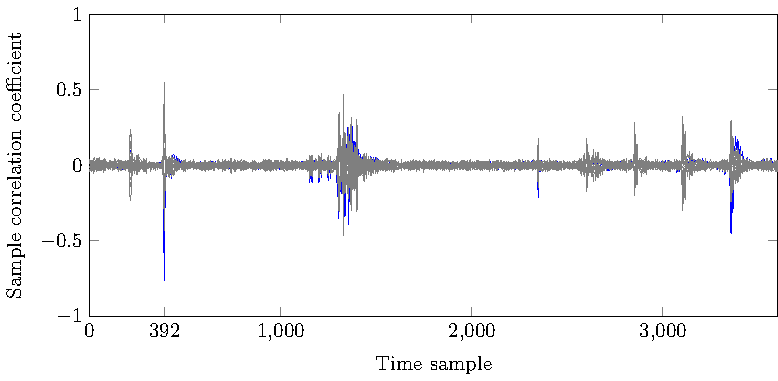
\includegraphics{fig/correlation_coefficients.pdf}
    \caption{Sample correlation coefficients $r_{i,t}$ ($i=1,2,\dots,16$) for all time samples $t=1,2,\dots,3600$.
    Computed with the identity leakage model and \dataranone.
    The blue line corresponds to the correct key hypothesis $\hat{k}_{10}=\texttt{9}$.}
\end{figure}
\end{frame}

\begin{frame}{DPA attack results -- Hamming weight leakage model}
    \begin{figure}[h]
    \centering
    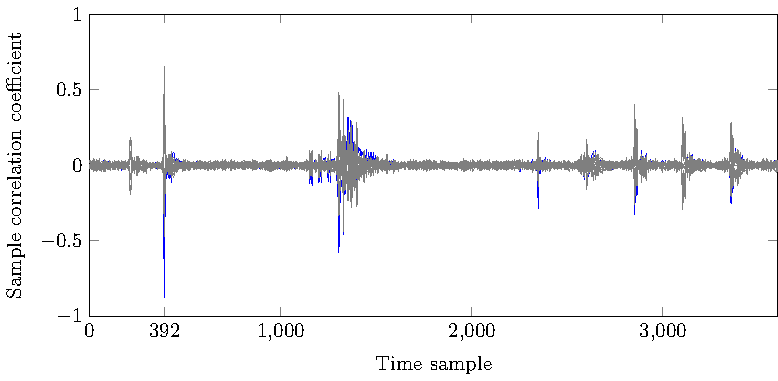
\includegraphics{fig/correlation_coefficient_hw.pdf}
    \caption{Sample correlation coefficients $r_{i,t}$ ($i=1,2,\dots,16$) for all time samples $t=1,2,\dots,3600$.
    Computed with the Hamming leakage model and \dataranone.
    The blue line corresponds to the correct key hypothesis $\hat{k}_{10}=\texttt{9}$.}
\end{figure}
\end{frame}

\begin{frame}{Remarks}
    \begin{itemize}
        \item The maximum absolute value of the correlation coefficient calculated using the identity leakage model is $0.7624$ for the correct key hypothesis, obtained at time sample $392$
        \item The maximum absolute value of the correlation coefficient calculated using the Hamming weight leakage model is $0.8747$ for the correct key hypothesis, obtained at time sample $392$
        \item The higher absolute correlation coefficient value for the Hamming weight leakage model indicates it is probably a better leakage model for our DUT compared to the identity leakage model
        \item We have seen in the last section that $392$ is the time sample that gives us the highest SNR value and also ``leaks'' the most according to TVLA
    \end{itemize}
\end{frame}

\begin{frame}{Remarks}
    \begin{itemize}
        \item Some peaks of $r_{i,t}$ corresponding to a wrong key hypothesis and the correct key hypothesis appear at similar time samples -- $\mathcal{H}_i$s are not independent random variables and for those time samples $t$, $\mathcal{H}_i$s also correlated with the actual leakage
        \item The correlation between $\mathcal{H}_i$s also influences the magnitude of the correlation coefficients for the wrong key hypotheses.
        If the correlation between $\mathcal{H}_i$s is higher, we would also see higher peaks in some wrong key hypotheses.
        For AES, the correlations between the first AddRoundKey outputs are higher than correlations between the first SubBytes operation outputs, that is why in step 4, we chose the target intermediate value to an Sbox output.
        \item The attacks we have seen recover one nibble of the first-round key.
        The other nibbles can be recovered independently with a similar method using the same traces.
    \end{itemize}
\end{frame}

\begin{frame}{Code}
    Implementation for attack using the identity leakage model can be found here
    \begin{center}
        \url{https://github.com/XIAOLUHOU/SCA-measurements-and-analysis----Experimental-results-for-textbook/blob/main/Assignment_materials/DPA.ipynb}
    \end{center}
\end{frame}